\chapter{Results and Analysis}

\section{Evaluation Setup}

We evaluated the full pipeline on synthetic query images from the Khumbu region. We used synthetic queries here because they give us exact ground truth camera locations, so location error can be measured directly without manual labelling.

For this preliminary evaluation stage, we used a reference database sampled on a regular 500\,m grid, which produced 4,920 viewpoints in the selected study area. Each viewpoint stores a precomputed skyline profile from the same \gls{dem} used in the database generation step.

To avoid confusion: 30\,m refers to \gls{dem} raster resolution, while 500\,m is the viewpoint sampling interval used in this initial Chapter 6 setup. This grid setting is not treated as final and will be refined in later stages.

\begin{table}[H]
\centering
\caption{Evaluation setup used in this chapter.}
\label{tab:evaluation_setup_results}
\begin{tabular}{ll}
\toprule
Parameter & Value\\
\midrule
Study area & Khumbu region, Nepal\\
Reference viewpoints (preliminary setup) & 4,920\\
Grid spacing (preliminary setup) & 500\,m\\
Query images & 300\\
Query type & Synthetic, grid-aligned\\
Ground truth & Known camera location\\
\bottomrule
\end{tabular}
\end{table}

All metrics reported in this chapter are measured under this preliminary setup: 300 synthetic queries, evaluated against the 500\,m reference grid used for this stage.

For this evaluation, skyline profiles are extracted using the ground-truth synthetic sky masks (Section 4.4.2) rather than masks predicted by the trained segmentation model. This isolates the accuracy of the skyline extraction and matching stages from segmentation error. End-to-end evaluation using predicted masks is planned as future work.

Figure~\ref{fig:horizon_database_preview} shows an example view from the reference skyline database.

\begin{figure}[H]
\centering
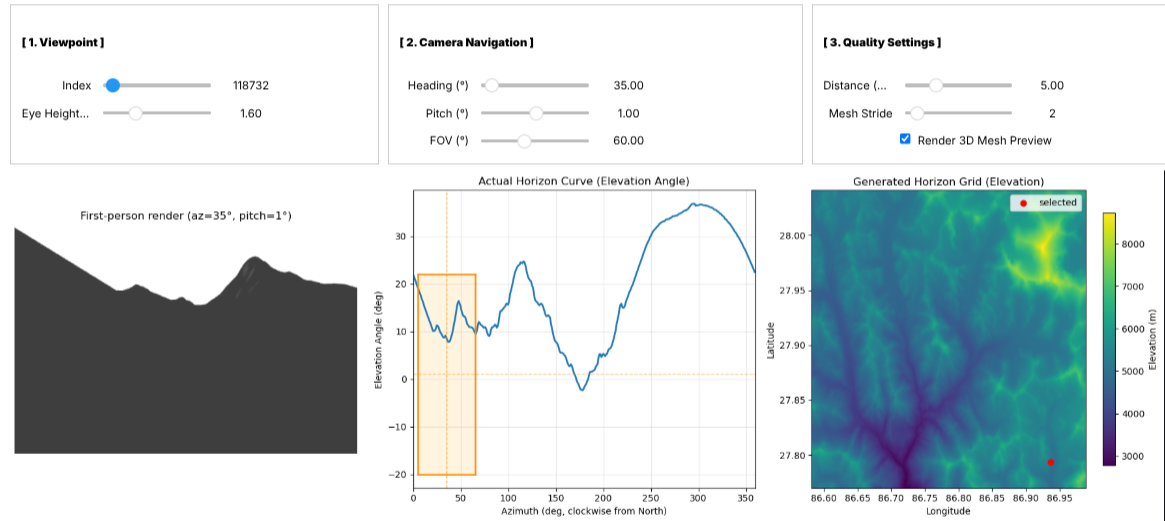
\includegraphics[width=0.9\textwidth]{src/images/horizon_database.png}
\caption{Reference skyline database preview used during matching.}
\label{fig:horizon_database_preview}
\end{figure}

\section{Synthetic Query Images}

The query set was generated by rendering synthetic mountain scenes under different lighting conditions and simple weather effects. This gives controlled variation while keeping exact camera metadata.

Figure~\ref{fig:synthetic_examples} shows sample synthetic query images used in testing.

\begin{figure}[H]
\centering
\begin{subfigure}[b]{0.82\textwidth}
\centering
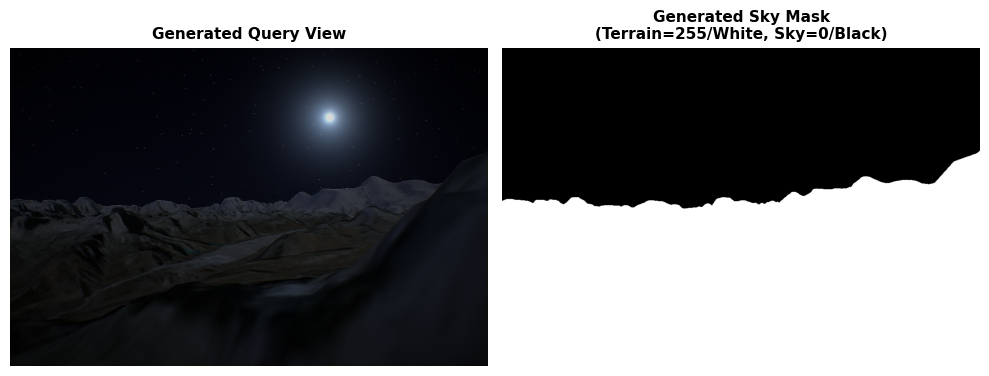
\includegraphics[width=\textwidth]{src/images/synthetic.png}
\caption{Synthetic sample A}
\end{subfigure}

\vspace{0.5em}

\begin{subfigure}[b]{0.82\textwidth}
\centering
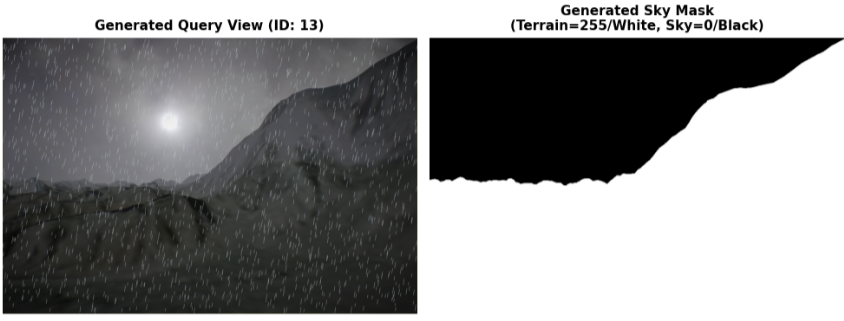
\includegraphics[width=\textwidth]{src/images/synthetic1.png}
\caption{Synthetic sample B}
\end{subfigure}

\vspace{0.5em}

\begin{subfigure}[b]{0.82\textwidth}
\centering
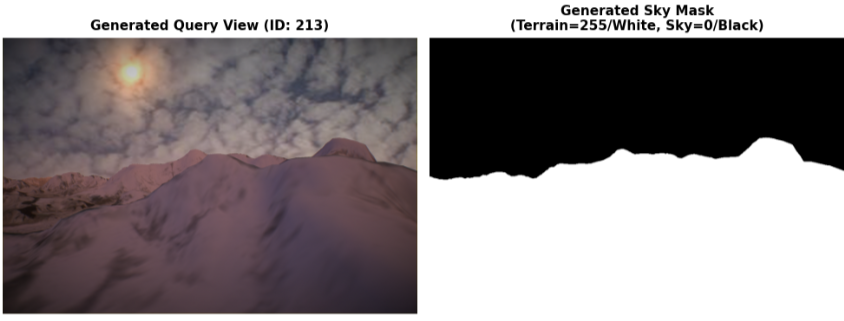
\includegraphics[width=\textwidth]{src/images/synthetic2.png}
\caption{Synthetic sample C}
\end{subfigure}
\caption{Examples of synthetic query images used for evaluation.}
\label{fig:synthetic_examples}
\end{figure}

\section{Segmentation Training Result}

We trained the skyline segmentation model for 15 epochs using GeoPose3K's predefined training split combined with our 300 synthetic images. We used transfer learning with a pretrained MobileNetV3 encoder. Figure~\ref{fig:unet_training_result} shows the training and validation curves from that run.

\begin{figure}[H]
\centering
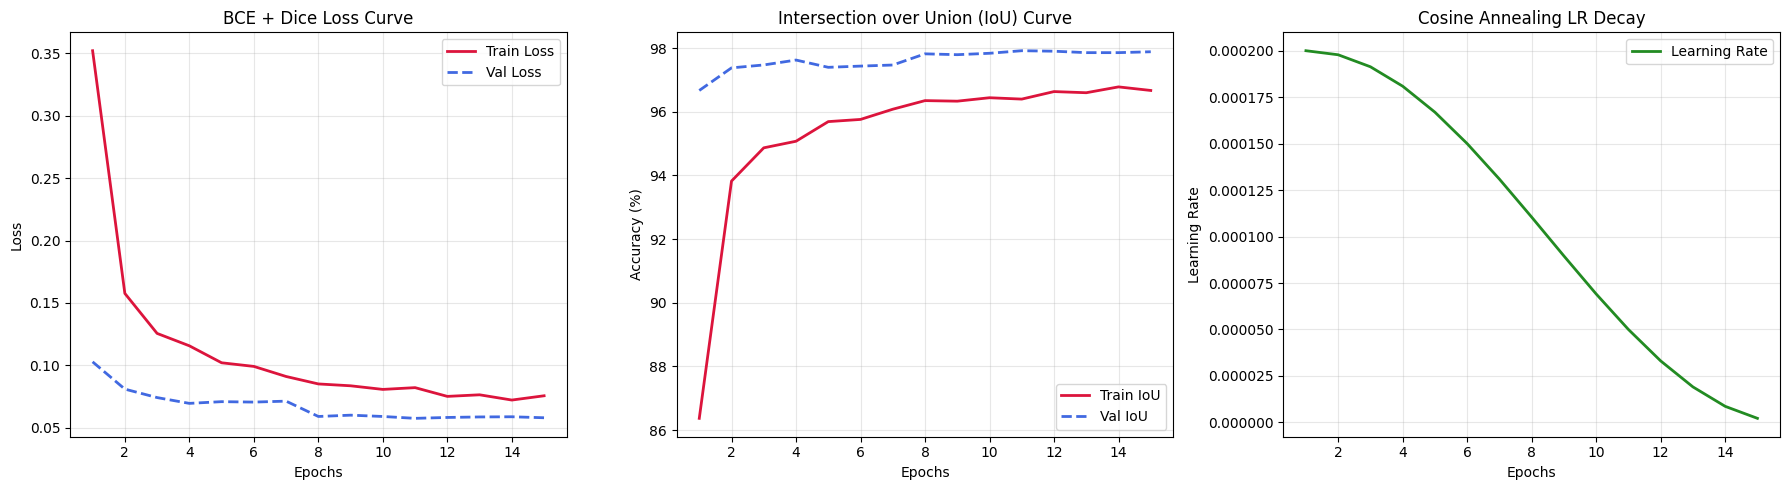
\includegraphics[width=\textwidth]{src/images/plot_unet.png}
\caption{Training and validation curves of the segmentation model.}
\label{fig:unet_training_result}
\end{figure}

Both training and validation loss decrease over epochs, and validation \gls{iou} stays high near the end of training. This means the model is learning the sky-terrain boundary under our mixed training setup (synthetic + GeoPose). During training, we also applied data augmentation to increase sample diversity. It still does not by itself prove the same quality on all real field photos, where haze, exposure, and foreground objects can differ from training data.

\section{Localization Accuracy}

Table~\ref{tab:localization_accuracy_final} reports localization accuracy for the same synthetic, grid-aligned query set described in Section~\ref{tab:evaluation_setup_results}.

\begin{table}[H]
\centering
\caption{Localization accuracy of the proposed system.}
\label{tab:localization_accuracy_final}
\begin{tabular}{lc}
\toprule
Metric & Result\\
\midrule
Accuracy @ 10\,m & 84.00\%\\
Accuracy @ 100\,m & 84.00\%\\
Accuracy @ 500\,m & 90.33\%\\
Accuracy @ 1000\,m & 94.67\%\\
Median error & 0.0\,m\\
Failed matches ($>$1000\,m) & 5.33\%\\
\bottomrule
\end{tabular}
\\[6pt]
\footnotesize\textit{Note:} Accuracy@10m and @100m are identical because predictions in this grid-aligned setup either land exactly on the correct viewpoint or miss by more than 100\,m (see Section 6.4.1). Median error of 0.0\,m reflects this same grid-alignment effect, not zero-error performance in general.
\end{table}

Figure~\ref{fig:accuracy_plot_final} shows the same values as a plot.

\begin{figure}[H]
\centering
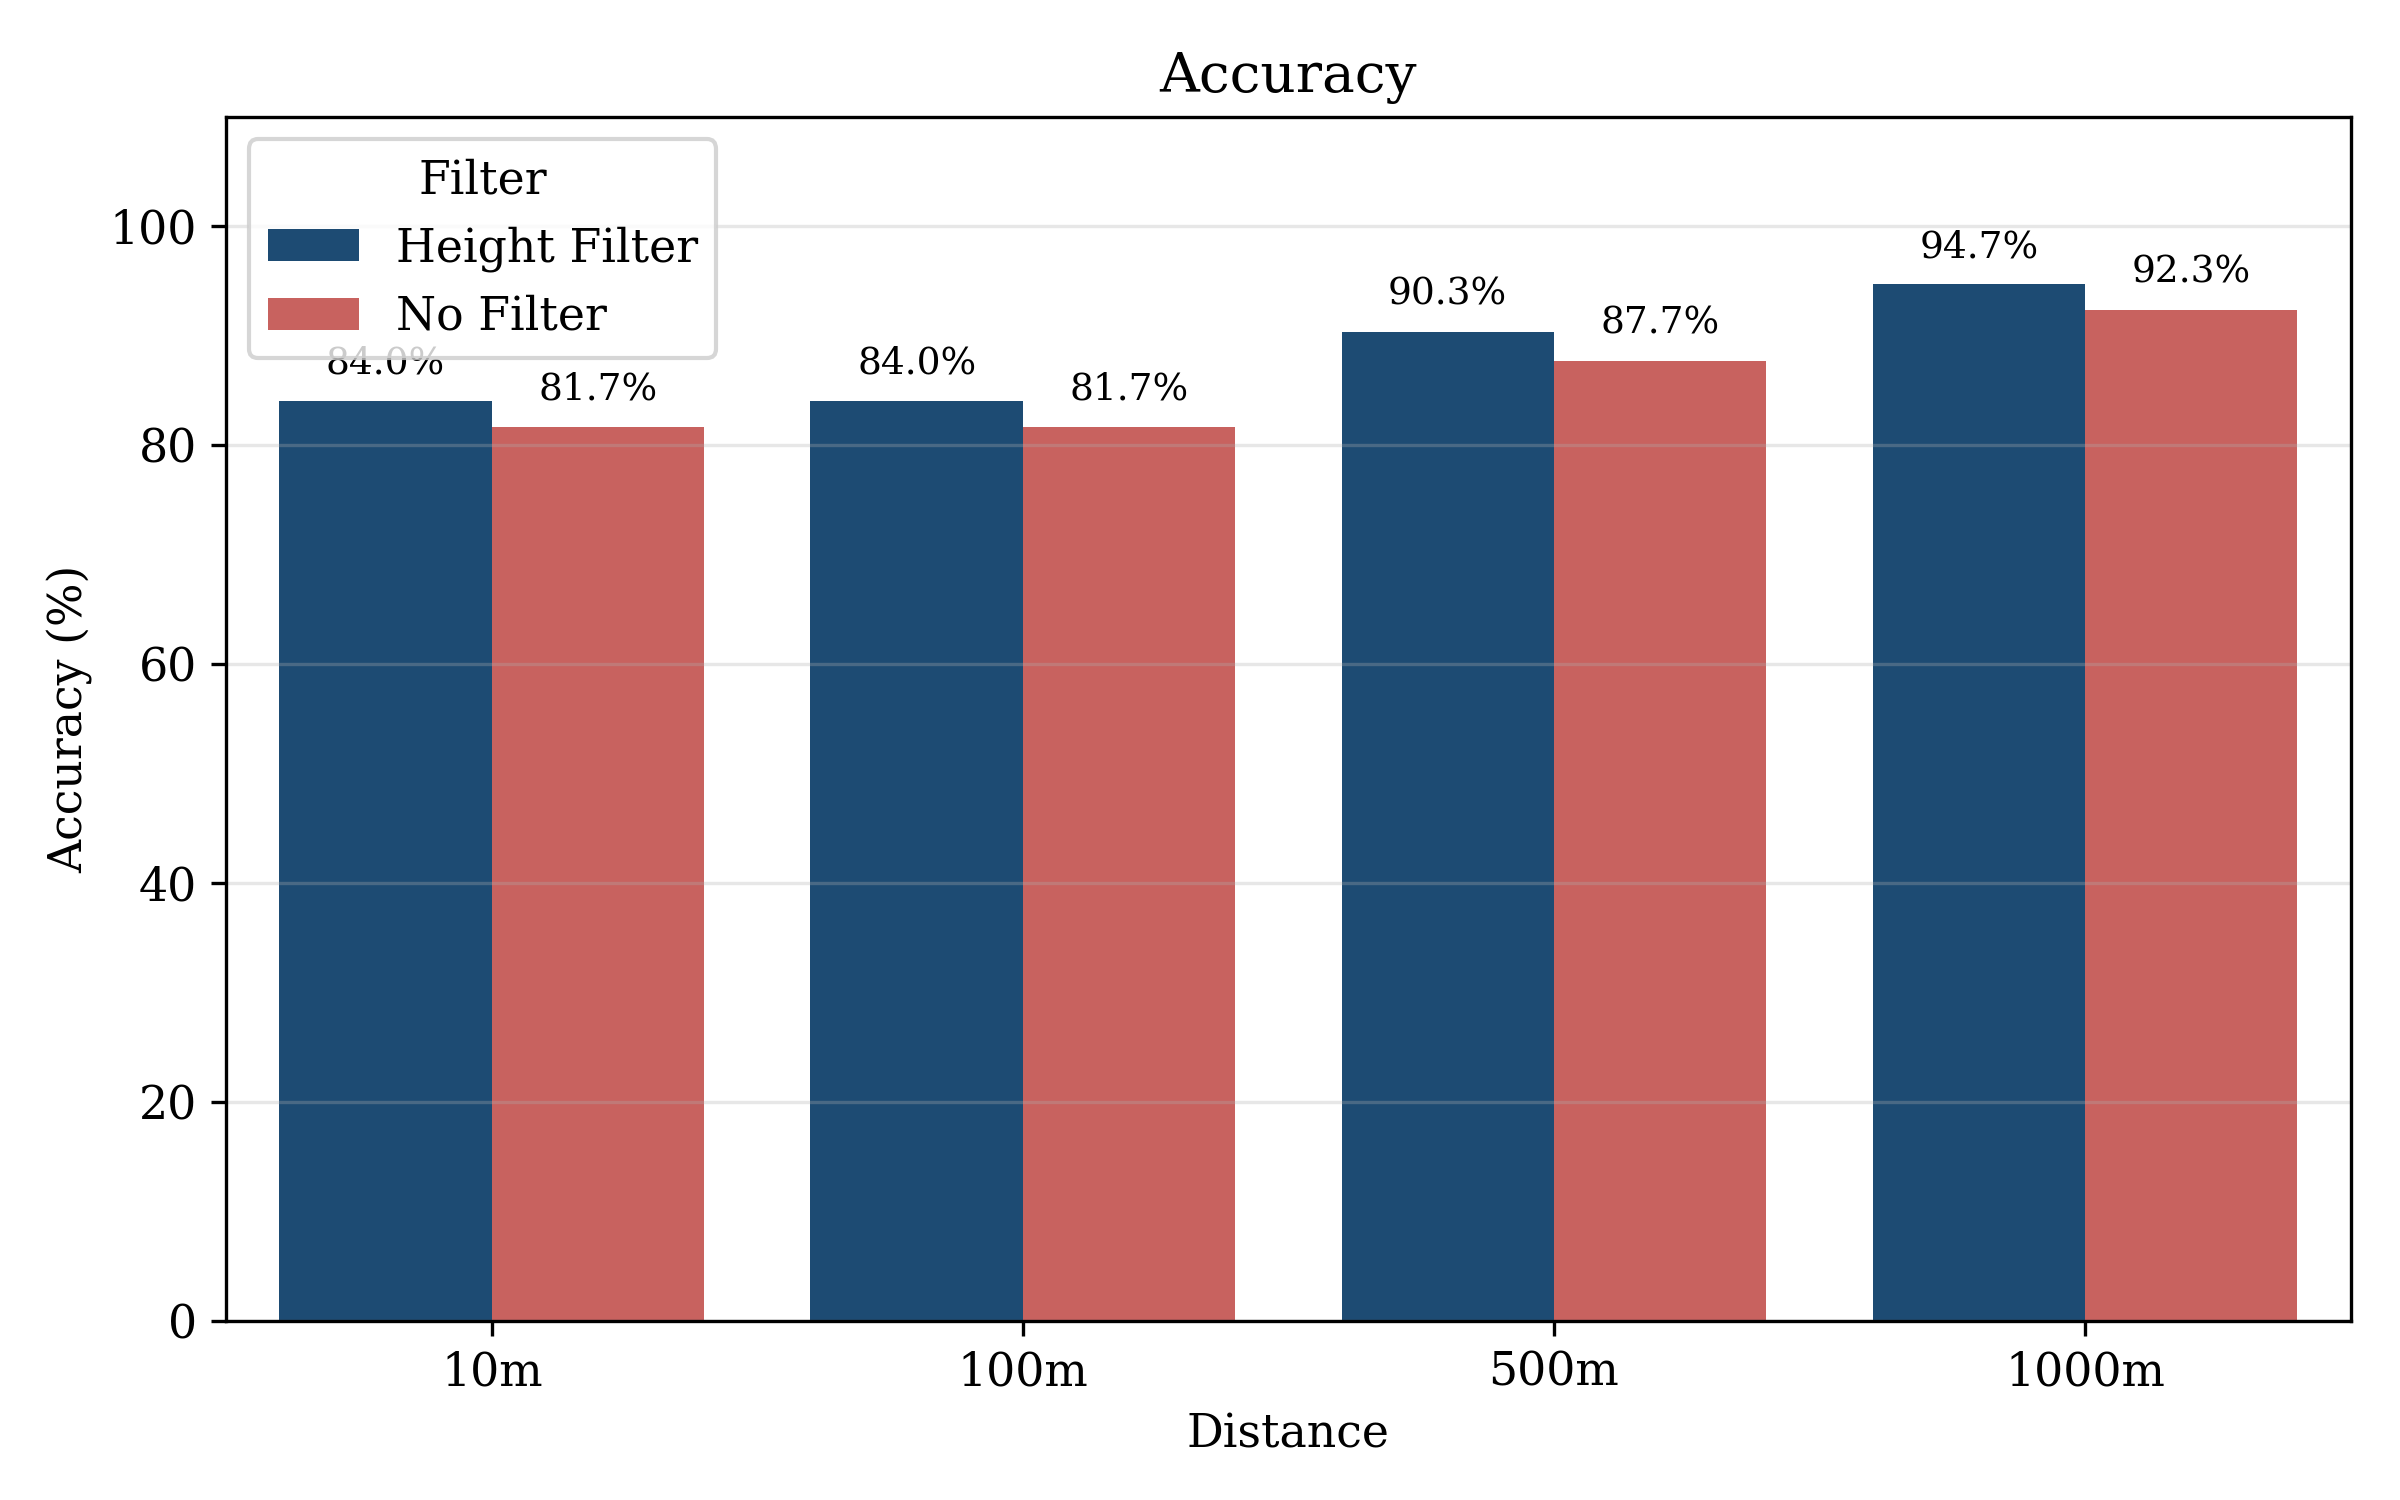
\includegraphics[width=0.75\textwidth]{src/images/plot_accuracy.png}
\caption{Localization accuracy at different distance thresholds.}
\label{fig:accuracy_plot_final}
\end{figure}

Figure~\ref{fig:accuracy_plot_final} also includes the result for optional height-filtered candidate pruning. In this experiment, reference viewpoints were restricted to a vertical window of \(\pm\)100\,m around the query elevation before skyline matching. Under the same grid-aligned synthetic setup, Top-1 accuracy at the 1000\,m threshold increased from 92.3\% to 94.7\%. This shows height filtering as a preliminary filtering stage that was experimentally evaluated, rather than the core localization method.

Out of 300 synthetic grid-aligned queries, 284 are localized within 1000\,m, 271 within 500\,m, and 252 within 100\,m.

The 10\,m and 100\,m values are both 84.00\% because of the test condition. In this dataset, many predictions either land exactly on the correct grid viewpoint or miss by more than 100\,m, so both thresholds count the same 252 samples.

The median error is 0.0\,m under this setup because at least half of the queries map exactly to the correct grid point. This is a side effect of grid-aligned testing, not a claim of zero-error behavior in free-position real-world use.

\subsection{Result Interpretation}

Figure~\ref{fig:accuracy_plot_final} and the qualitative examples in Figure~\ref{fig:qualitative_examples} are both measured on grid-aligned synthetic queries sampled from the same grid family as the reference database. These results therefore represent a favorable matching condition. Off-grid accuracy is not measured in this chapter.

If a user stands between grid points (for example, near the midpoint between neighboring samples), localization can degrade because no reference point is exactly at that location. However, distant mountain peaks are usually several kilometers away, so moderate horizontal shifts produce limited angular skyline change. The \gls{dtw} refinement step helps handle these small local distortions by allowing non-rigid alignment rather than strict point-to-point matching.

\subsection{Evaluation Limitations}

This evaluation has four key limitations. First, all queries are grid-aligned synthetic views, so off-grid behavior is not measured. Second, camera tilt is not varied; all queries use horizontal orientation, while real users often tilt the camera up or down. Third, the images are synthetic with relatively clear sky boundaries, whereas real photos may include haze, cloud, and foreground clutter that make skyline extraction harder. Fourth, localization accuracy is evaluated using ground-truth sky masks rather than segmentation model predictions, so these results do not include segmentation error. Combining the trained segmentation model with the matching pipeline for full end-to-end evaluation is the next planned step. A deeper error analysis across terrain and image conditions remains future work.

\section{Qualitative Examples}

Figure~\ref{fig:qualitative_examples} shows two representative localization outputs.

\begin{figure}[H]
\centering
\begin{subfigure}[b]{0.9\textwidth}
\centering
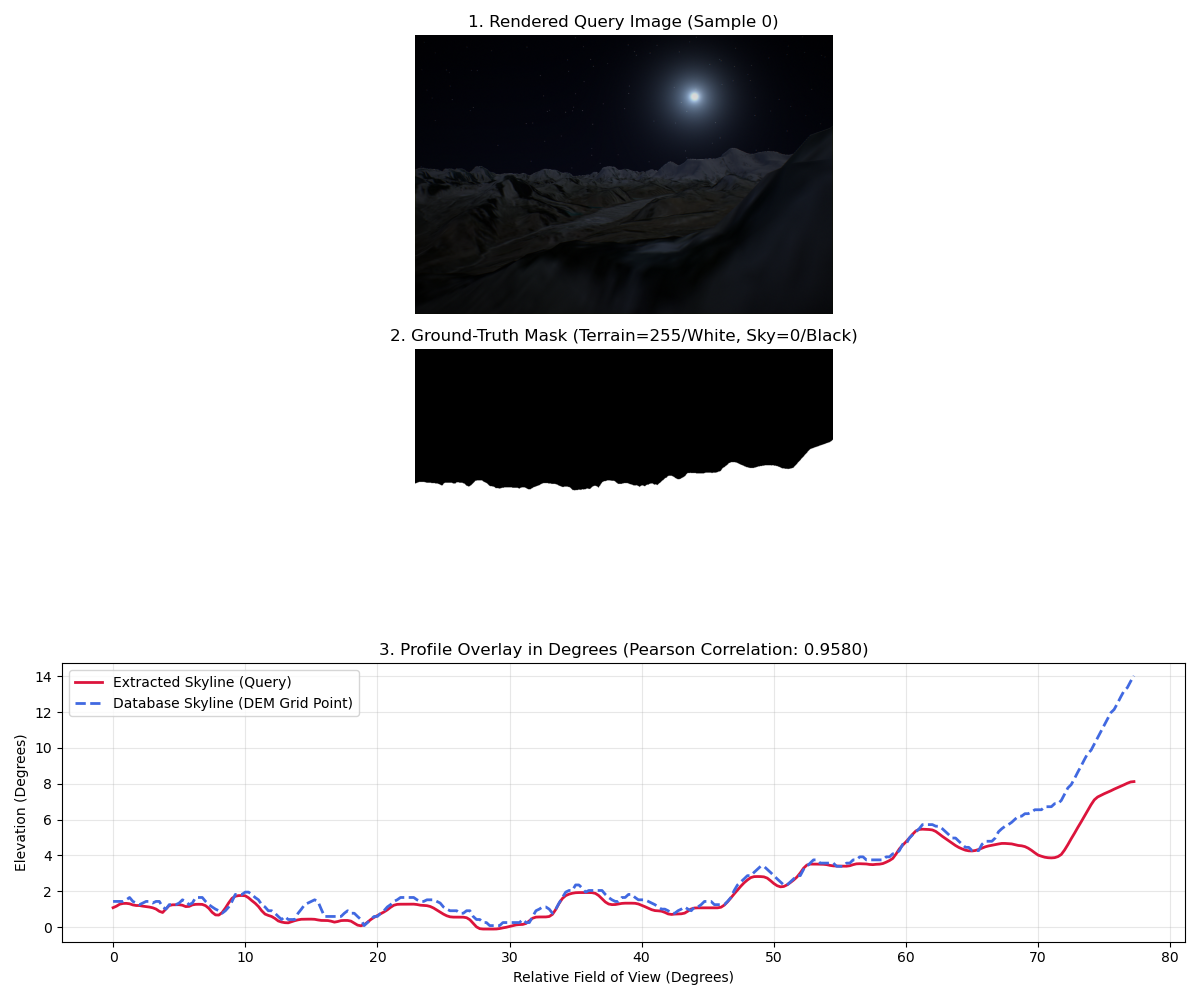
\includegraphics[width=\textwidth]{src/images/visualize0.png}
\caption{Sample 0}
\end{subfigure}

\vspace{0.6em}

\begin{subfigure}[b]{0.9\textwidth}
\centering
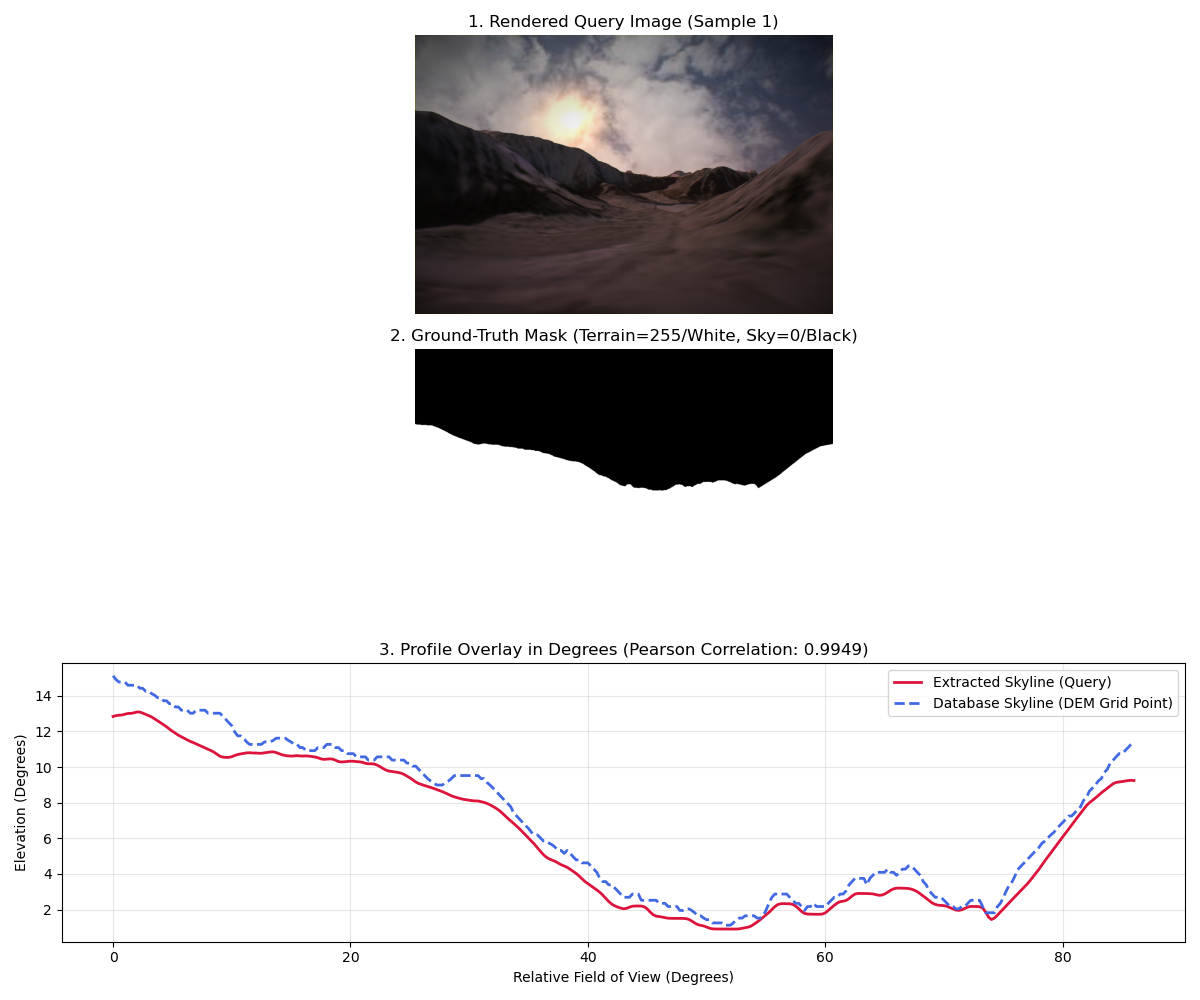
\includegraphics[width=\textwidth]{src/images/visualize1.png}
\caption{Sample 1}
\end{subfigure}

\caption{Representative localization visualizations from the grid-aligned test set.}
\label{fig:qualitative_examples}
\end{figure}

In successful cases, the predicted skyline shape matches the reference shape at the main peaks and valleys. In failed cases, the skyline still looks visually similar, but a nearby wrong candidate receives a higher score.

The failure rate in this test is 5.33\% (16 out of 300, from the ``Failed matches ($>$1000\,m)'' row in Table~\ref{tab:localization_accuracy_final}). In inspected failed examples, two patterns are commonly observed:

\begin{enumerate}
\item Low skyline contrast in difficult weather or lighting, which makes boundary extraction less stable.
\item Repeated ridge geometry, where different viewpoints produce similar skyline profiles.
\end{enumerate}

This explains why some failures are not random noise but structured confusion between look-alike terrain profiles.

\section{Summary}

The system performs well on this synthetic grid-aligned benchmark using ground-truth sky masks: 94.67\% of queries are within 1\,km and 90.33\% are within 500\,m; end-to-end accuracy with predicted segmentation masks has not yet been measured.
Because the database spacing is 500\,m, a 1\,km error corresponds to approximately two grid cells.
This helps interpret the 1000\,m metric in terms of the reference sampling geometry.

These numbers should not be read as final field performance. They are measured on synthetic data with known camera states and grid-aligned viewpoints. Real-world testing will need off-grid captures, and stronger environmental variation before we can claim deployment-level accuracy.
